
\def\theradius{1.75cm}

\begin{figure}[ht]

  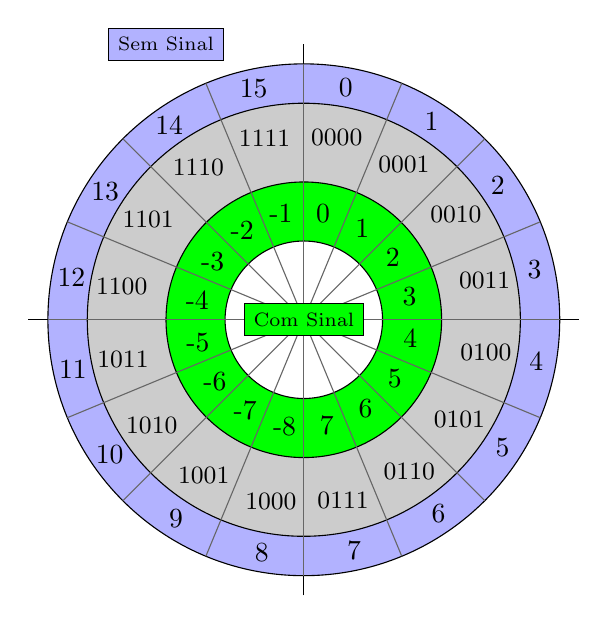
\begin{tikzpicture}[
    theguide/.style={draw opacity=0,very thin}
    ]
    
    \draw (-2*\theradius,0) -- (2*\theradius,0);
    \draw (0,-2*\theradius) -- (0,2*\theradius);
    \draw[fill=blue!30] (0,0) circle (\theradius+1.5cm);
    \draw[fill=gray!40] (0,0) circle (\theradius+1cm);
    \draw[fill=green] (0,0) circle (\theradius);
    \draw[fill=white] (0,0) circle (\theradius-.75cm);
    
    \foreach \i/\b/\s in {0/0000/0,1/0001/1,2/0010/2,3/0011/3,4/0100/4,
      5/0101/5,6/0110/6,7/0111/7,8/1000/-8,9/1001/-7,10/1010/-6,11/1011/-5,
      12/1100/-4,13/1101/-3,14/1110/-2,15/1111/-1} {
      \draw[draw=black!60] (0,0) -- (\s*22.5:\theradius+1.5cm);
      \draw[theguide] (0,0) -- (\i*-22.5+79.75:\theradius+1.25cm)
      node[] {\i};
      \draw[theguide] (0,0) -- (\i*-22.5+79.75:\theradius+.6cm)
      node {\small \b};
      \draw[theguide] (0,0) -- (\i*-22.5+79.75:\theradius-.375cm)
      node {\s};
    }
    \node[draw,fill=blue!30] at (-\theradius, 2*\theradius) {\scriptsize Sem Sinal};
    \node[draw,fill=green] at (0,0) {\scriptsize Com Sinal};
  \end{tikzpicture}

  \label{fig:4bits:circle}
  \caption{}
\end{figure}
